%%%%%%%%%%%%%%%%%%%%%%%%%%%%%%%%%%%%%%%%%%%%%%%%%%%%%%%%%%%%%%%%%%%%%%%%%%%  BASIC  %%%%%%%%%%%%%%%%%%%%%%%%%%%%%%%%%%%%%%%%%%%%%%%%%%%%%%%%%%%%%%%%%%%%%%%%%%%

\section{Basic}

\subsection{Default code}
\lstinputlisting{basic/Default.cpp}

\subsection{Misc}
\lstinputlisting{basic/Misc.cpp}

\subsection{Fast read \& write}
\lstinputlisting{basic/FastRW.cpp}

\subsection{Sort cmp}
\lstinputlisting{basic/Cmp.cpp}

\subsection{Discretization}
\lstinputlisting{basic/Discretization.cpp}

\subsection{Custom unordered\_map}
\lstinputlisting{basic/CustomUnordered\_map.cpp}

\subsection{\_\_int128 read}
\lstinputlisting{basic/Int128IO.cpp}

\subsection{字典序a嚴格小於b}
\lstinputlisting{basic/LexicographicallySmaller.cpp}

\subsection{Radom}
\lstinputlisting{basic/Random.cpp}

%%%%%%%%%%%%%%%%%%%%%%%%%%%%%%%%%%%%%%%%%%%%%%%%%%%%%%%%%%%%%%%%%%%%%%%%%%%  Matching  %%%%%%%%%%%%%%%%%%%%%%%%%%%%%%%%%%%%%%%%%%%%%%%%%%%%%%%%%%%%%%%%%%%%%%%%%%%
\section{對拍}

\subsection{run.bat}
\lstinputlisting{matching/run.bat}

\subsection{run.sh}
\lstinputlisting{matching/run.sh}
%%%%%%%%%%%%%%%%%%%%%%%%%%%%%%%%%%%%%%%%%%%%%%%%%%%%%%%%%%%%%%%%%%%%%%%%%%%  Flow  %%%%%%%%%%%%%%%%%%%%%%%%%%%%%%%%%%%%%%%%%%%%%%%%%%%%%%%%%%%%%%%%%%%%%%%%%%%
\section{Flow \& Matching}

\subsection{Dicnic}
\lstinputlisting{flow/Dicnic.cpp}

\subsection{ZKW FLow}
\lstinputlisting{flow/ZkwFlow.cpp}

\subsection{Hungarian}
\lstinputlisting{flow/Hungarian.cpp}

\subsection{KM}
\lstinputlisting{flow/KM.cpp}

%%%%%%%%%%%%%%%%%%%%%%%%%%%%%%%%%%%%%%%%%%%%%%%%%%%%%%%%%%%%%%%%%%%%%%%%%%%  Graph  %%%%%%%%%%%%%%%%%%%%%%%%%%%%%%%%%%%%%%%%%%%%%%%%%%%%%%%%%%%%%%%%%%%%%%%%%%%
\section{Graph}

\subsection{BCC}
\lstinputlisting{graph/BccVertex.cpp}

\subsection{SCC}
\lstinputlisting{graph/SCC.cpp}

\subsection{2SAT}
\lstinputlisting{graph/2SAT.txt}

\subsection{MaximalClique}
\lstinputlisting{graph/MaximalClique.cpp}

\subsection{MaximumClique}
\lstinputlisting{graph/MaximumClique.cpp}

\subsection{Minimum Mean Cycle}
\lstinputlisting{graph/Minimum Mean Cycle.cpp}

\subsection{Dominator Tree}
\lstinputlisting{graph/Dominator Tree.cpp}


%%%%%%%%%%%%%%%%%%%%%%%%%%%%%%%%%%%%%%%%%%%%%%%%%%%%%%%%%%%%%%%%%%%%%%%%%%%  Math  %%%%%%%%%%%%%%%%%%%%%%%%%%%%%%%%%%%%%%%%%%%%%%%%%%%%%%%%%%%%%%%%%%%%%%%%%%%
\section{Math}

\subsection{Formulas}
\lstinputlisting{math/Formula.txt}

\subsection{Quick Pow}
\lstinputlisting{math/QuickPow.cpp}

\subsection{Mat quick Pow}
\lstinputlisting{math/MatPow.cpp}

\subsection{Primes Table}
\lstinputlisting{math/PrimesTable.cpp}

\subsection{Factor Table}
\lstinputlisting{math/FactorTable.cpp}

\subsection{Catalan Number}
\lstinputlisting{math/CatalanNumber.cpp}

\subsection{Miller Rabin}
\lstinputlisting{math/MillerRabin.cpp}

\subsection{PollarRho}
\lstinputlisting{math/PollardRho.cpp}

\subsection{PrimeFactorO(logn)}
\lstinputlisting{math/PrimeFactorO(logn).cpp}

\subsection{O(1)mul}
\lstinputlisting{math/O(1)mul.cpp}

\subsection{Josephus Problem}
\lstinputlisting{math/JosephusProblem.cpp}

\subsection{Harmonic Sum}
\lstinputlisting{math/HarmonicSum.cpp}

%%%%%%%%%%%%%%%%%%%%%%%%%%%%%%%%%%%%%%%%%%%%%%%%%%%%%%%%%%%%%%%%%%%%%%%%%%%  DataStructure  %%%%%%%%%%%%%%%%%%%%%%%%%%%%%%%%%%%%%%%%%%%%%%%%%%%%%%%%%%%%%%%%%%%%%%%%%%%
\section{Data Structure}

\subsection{BIT}
\lstinputlisting{math/BIT.cpp}

\subsection{Sparse Table}
\lstinputlisting{math/Sparse Table.cpp}

\subsection{Segment Tree}
\lstinputlisting{math/SegmentTree.cpp}

\subsection{Time Segment Tree}
\lstinputlisting{math/TimeSegmentTree.cpp}

\subsection{Treap}
\lstinputlisting{math/Treap.cpp}

\subsection{PBDS}
\lstinputlisting{math/PBDS.cpp}
%%%%%%%%%%%%%%%%%%%%%%%%%%%%%%%%%%%%%%%%%%%%%%%%%%%%%%%%%%%%%%%%%%%%%%%%%%%  Python  %%%%%%%%%%%%%%%%%%%%%%%%%%%%%%%%%%%%%%%%%%%%%%%%%%%%%%%%%%%%%%%%%%%%%%%%%%%
\section{Python}

\subsection{Decimal}
\lstinputlisting{python/Decimal.py}

\subsection{Fraction}
\lstinputlisting{python/Fraction.py}

\subsection{Misc}
\lstinputlisting{python/Misc.py}
\onecolumn
\centering
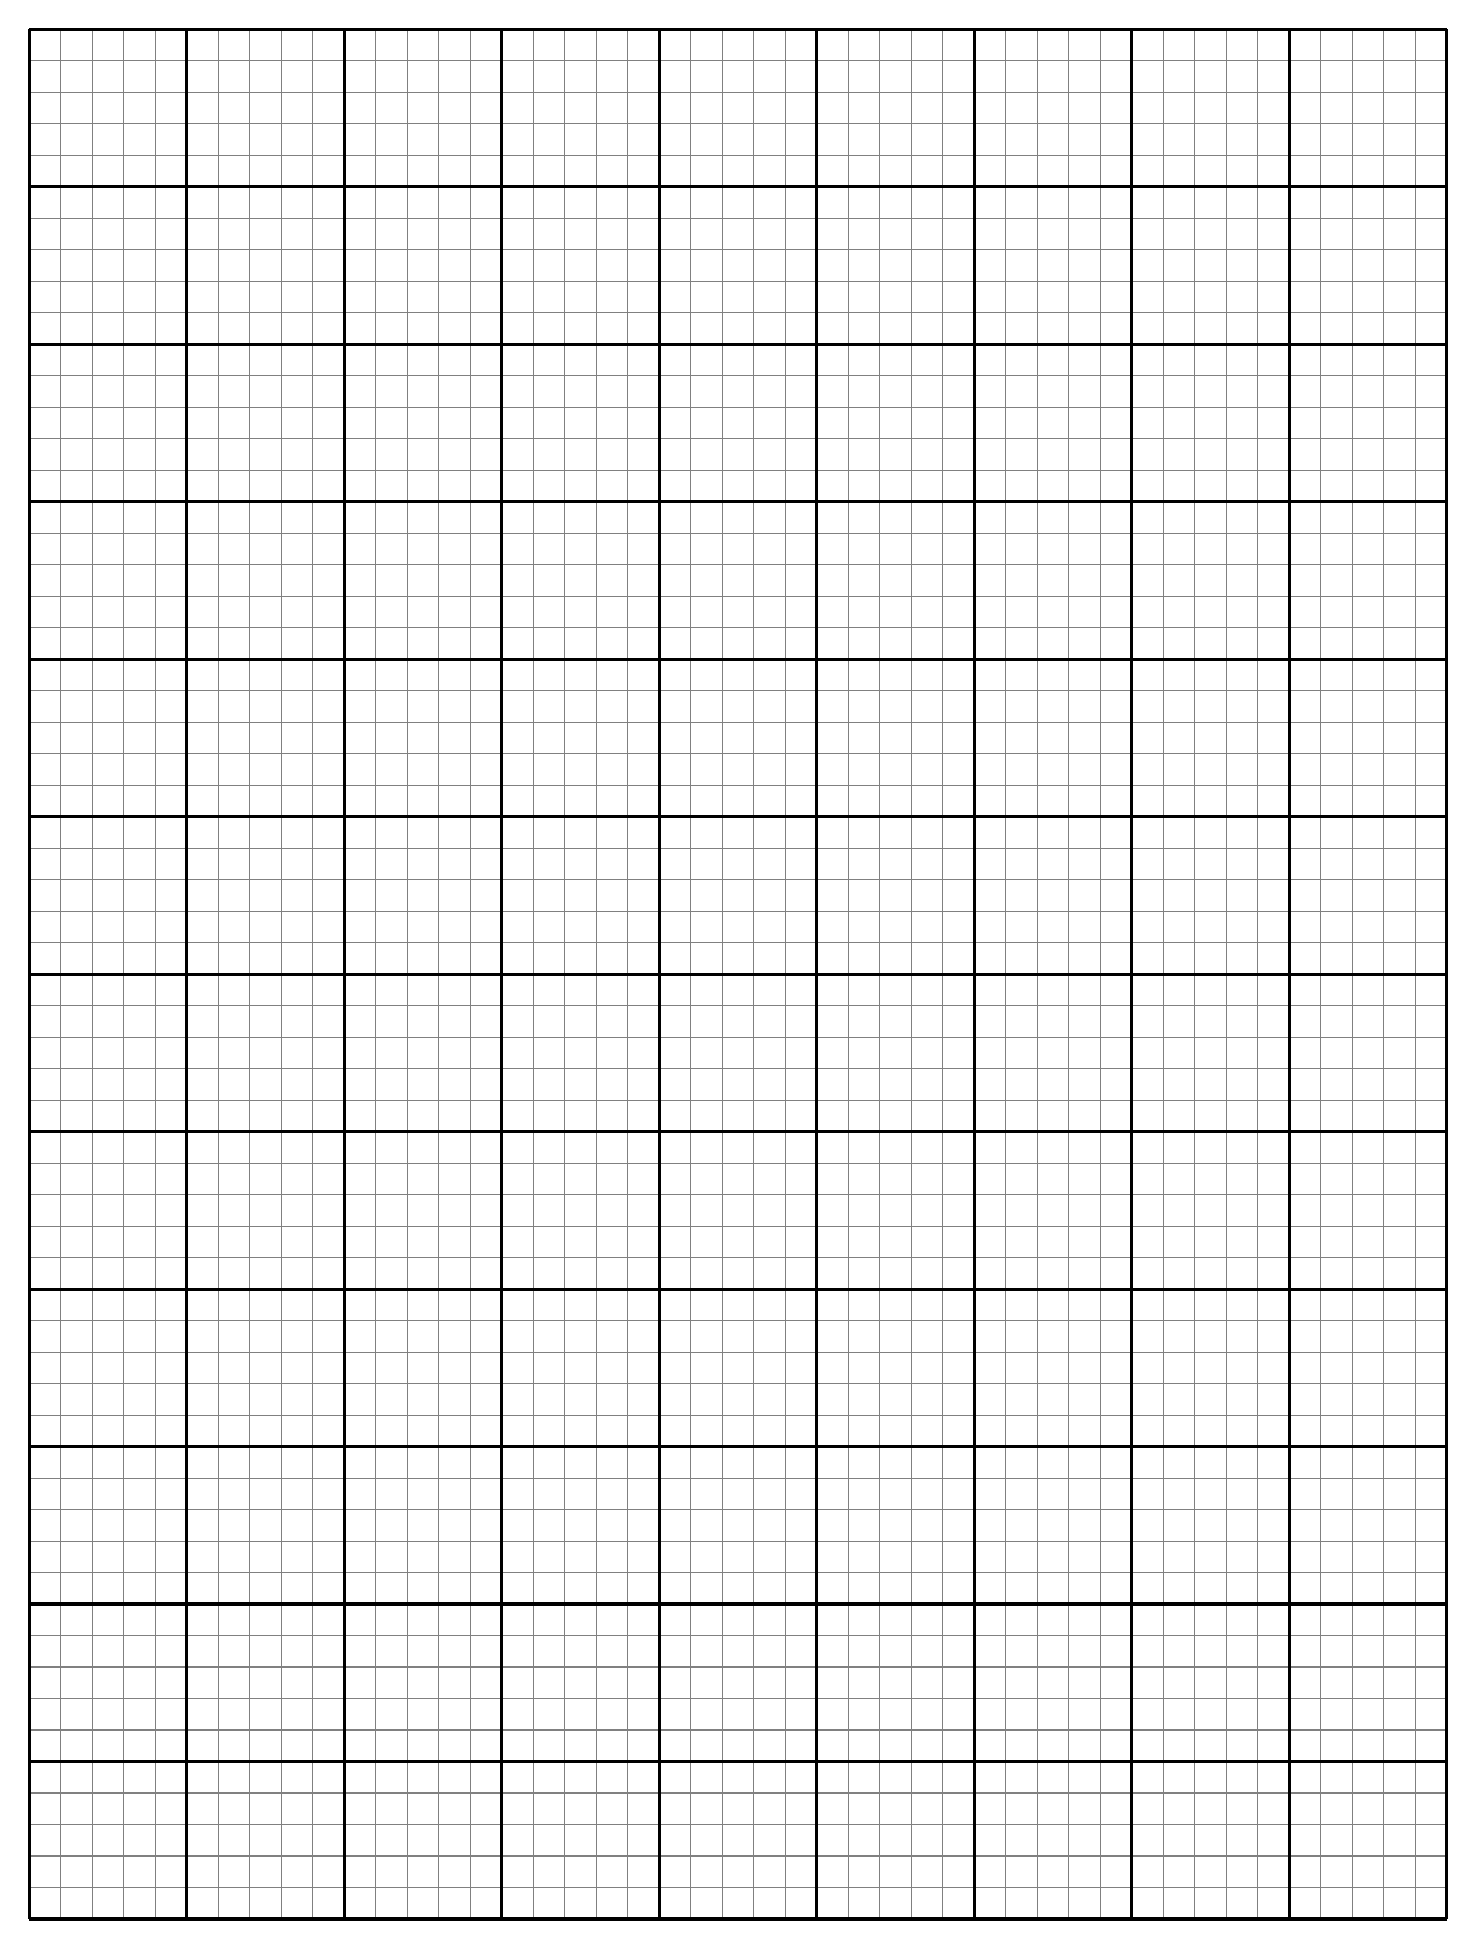
\begin{tikzpicture}[every node/.style={minimum size=1cm-\pgflinewidth, outer sep=10pt}, scale=2]
    \draw[step=0.2cm,color=gray] (0,0) grid (9,12);
    \draw[step=1cm,color=black,line width=0.4mm] (0,0) grid (9,12);
\end{tikzpicture}

\centering
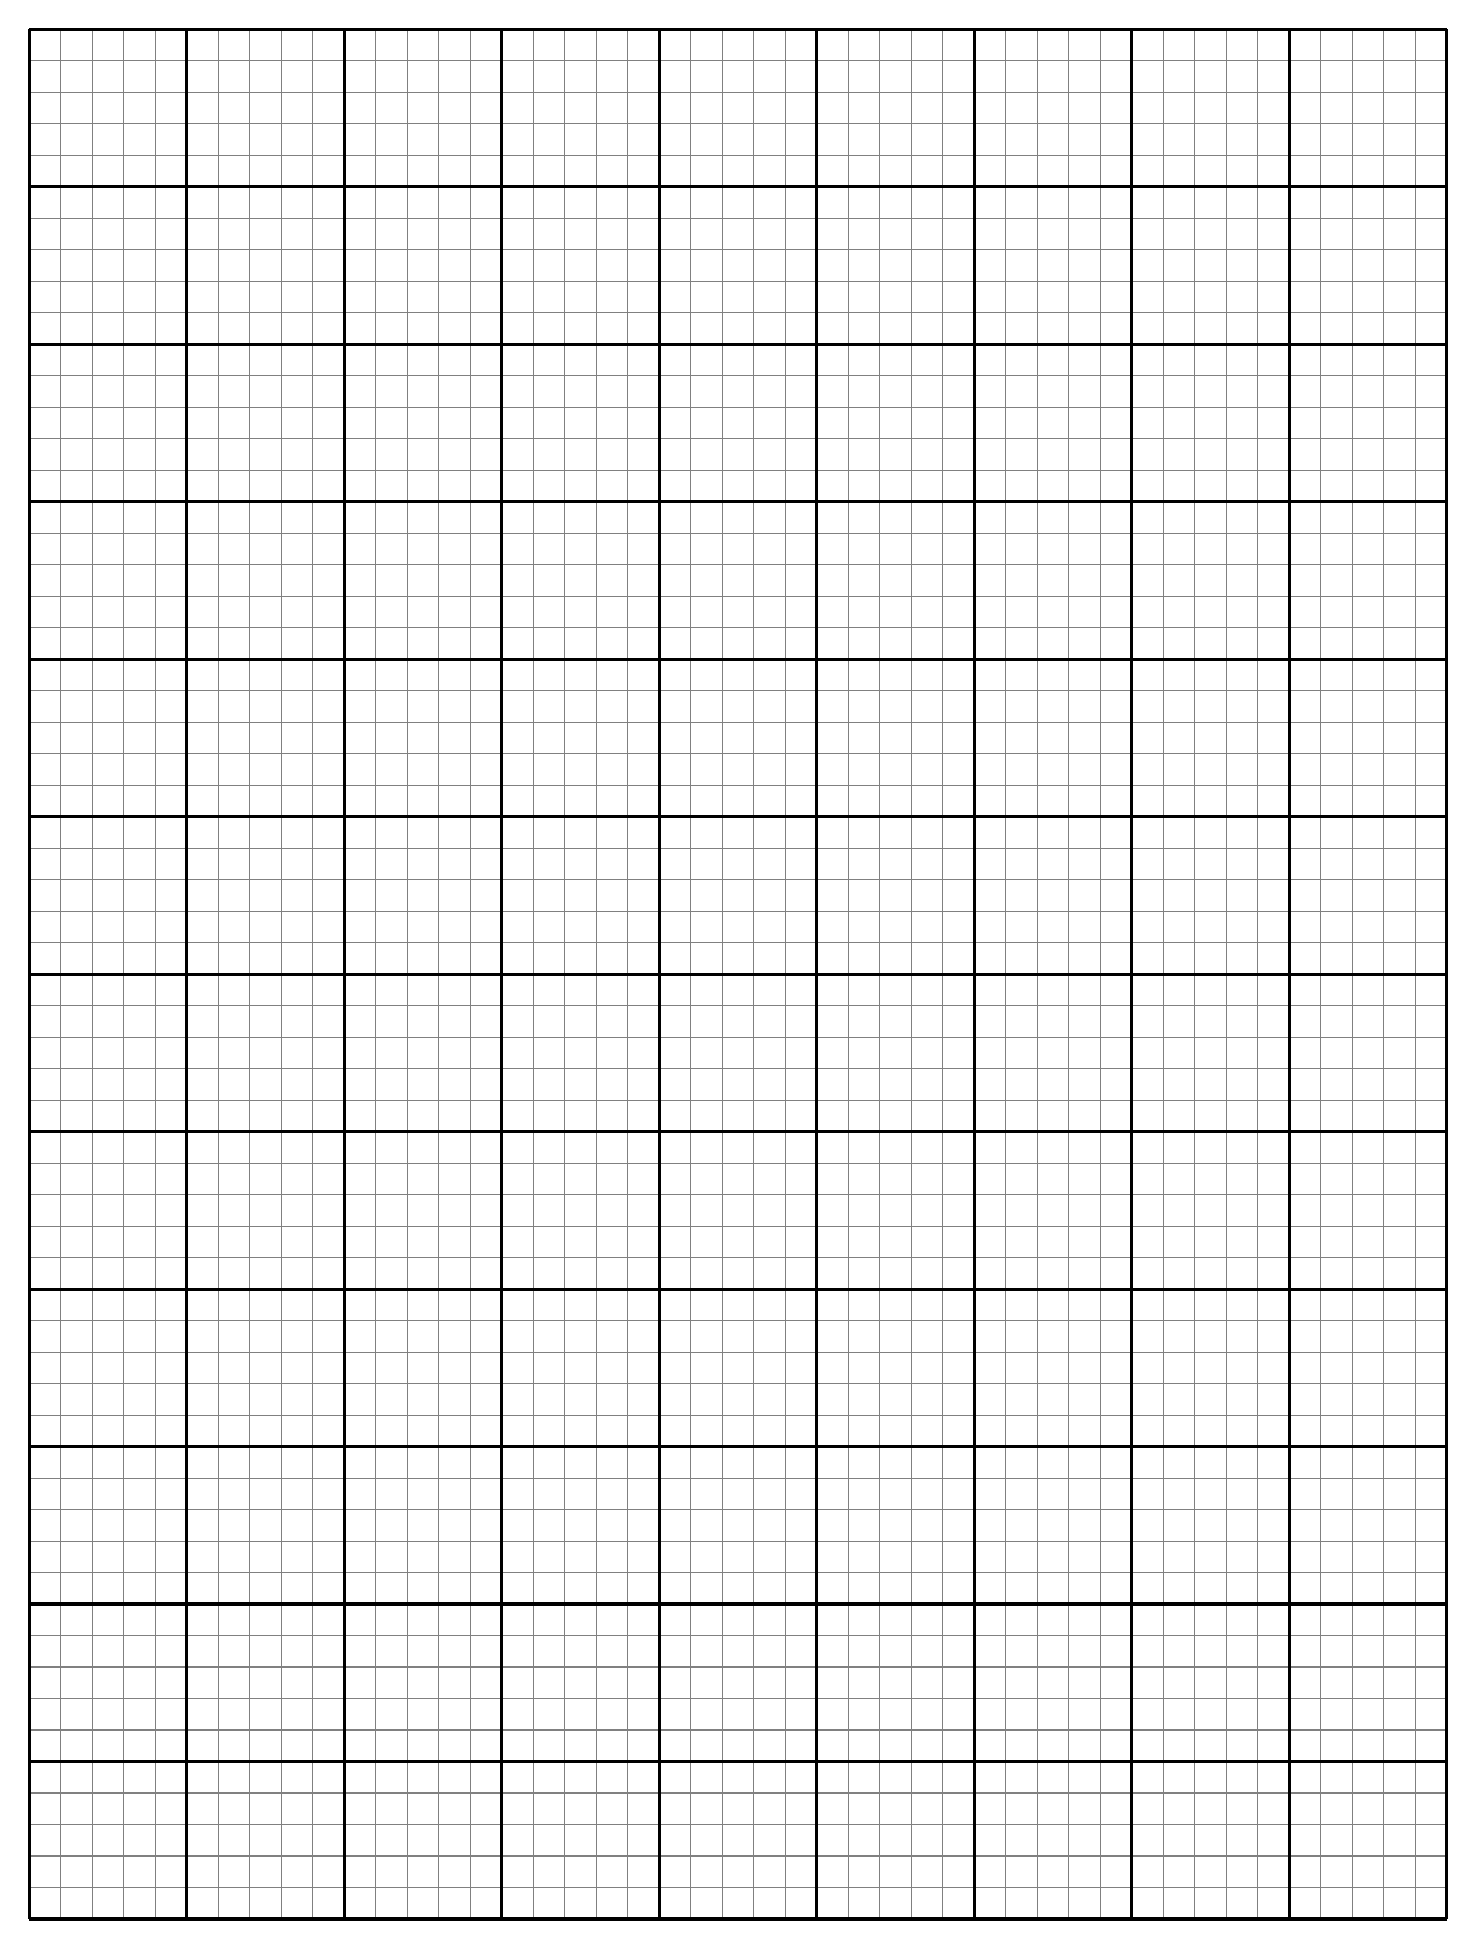
\begin{tikzpicture}[every node/.style={minimum size=1cm-\pgflinewidth, outer sep=10pt}, scale=2]
    \draw[step=0.2cm,color=gray] (0,0) grid (9,12);
    \draw[step=1cm,color=black,line width=0.4mm] (0,0) grid (9,12);
\end{tikzpicture}